\chapter{Continuous Static Analysis}
\label{cap:continuous_static_analysis}

In Free Software projects, a common source of bug reports are the GNU/Linux
distributions. These distributions ship thousands of software projects, which
they call packages. Distribution developers refer to the developers and
maintainers of the software they ship in the distribution as \textit{upstream}.
Distribution packages are used by a significant amount of users who, by using
such packages, often find bugs in them. As shown in Figure
\ref{fig:floss_bugs_workflow}, the users report the bugs they find to the
distribution developers, who in turn report these bugs to the upstream of the
package in which bugs were found.

\begin{figure}[!h]
  \centering
  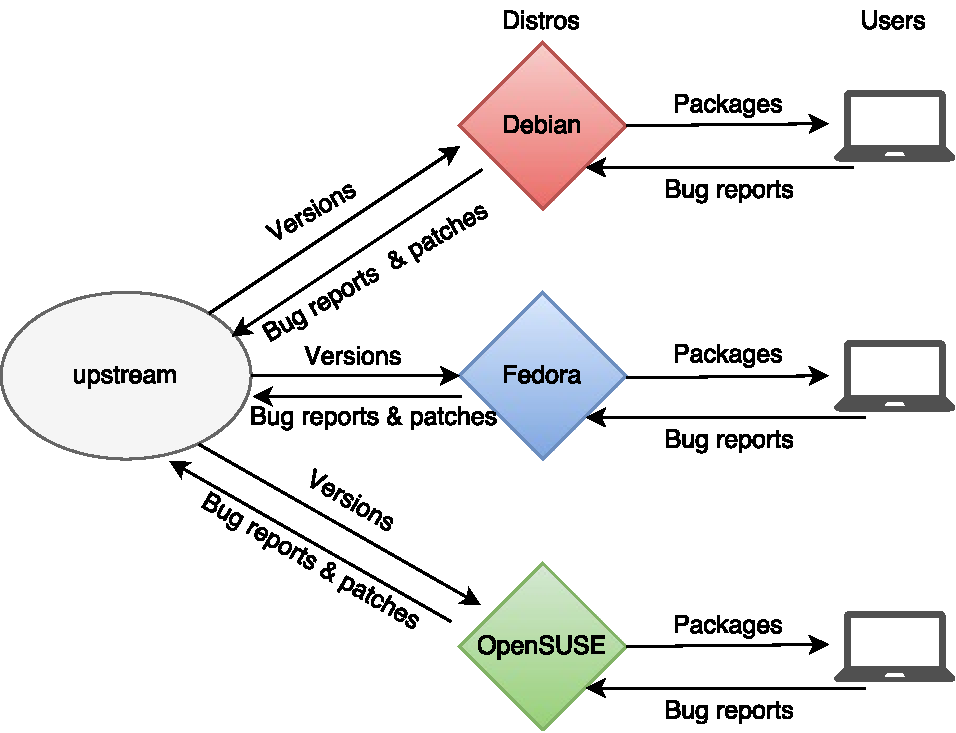
\includegraphics[width=.60\textwidth]{figures/floss_bugs_workflow} 
  \caption{FLOSS bug report workflow.}
  \label{fig:floss_bugs_workflow} 
\end{figure}

By continuously running multiple static analyzers in several of these packages,
i.e., once for each version of the package, we want to create a
database of static analysis reports on software of different sizes and
application domains, which could finally be used to train and validate methods
to rank warnings. Note that we chose to use GNU/Linux distributions due to the
high amount of software packages available and the well-defined and documented
interfaces they provide to download the latest versions of these packages. We
could also have used other sources such as git forges like
\textit{github}\footnote{\url{github.com}} or
\textit{gitlab}\footnote{\url{gitlab.com}} that also have a considerable number
of software available (we will provide a plugin interface that will make it possible to
implement this feature in the future), but since the cultural norm for
GNU/Linux distributions developers is to report (and often propose fixes for)
bugs, using their repositories for this work may provide a larger user base for
the tools developed in this research.

\textit{kiskadee} is the system proposed in Section
\ref{sec:contributions} as Contribution 1, which performs continuous static analysis of the
distribution packages. While the system details and architecture are discussed
in Section \ref{sec:kiskadee}, its features are described below:

\begin{enumerate}
\item \textbf{Monitor specific software repositories for new releases.} This\
way, we can track and analyze each release of the monitored packages since we\
started monitoring them.

\item \textbf{Download new software packages from the repositories.}

\item \textbf{Run multiple static analyzers on the downloaded packages.}

\item \textbf{Translate each static analyzer report to a common report format.} This\
is needed to enable analyzing the reports during the ranking and visualization\
phase. Since the system is extensible, we do not want to write parsing\
rules for each static analyzer report format to compare the analyzers, so we do\
this before saving the static analysis output.

\item \textbf{Save the reports in a database.}
\end{enumerate}

With \textit{kiskadee} in production, we will study the information collected
in the database to elaborate, train, test, and apply appropriate methods to
rank all the warnings reported for a given version of a package (more details
in Section \ref{sec:ranking_warnings}), based on information like:

\begin{itemize}
  \item Metrics based on false positive, true positive, and false negative rates of each tool that triggered a warning.

  \item Criticality of the CWEs related to each warning.

  \item Redundancy of warnings in the database (different tools may raise the\
    same warning).

  \item Additional validation to check whether a given warning is a bug or a false positive based on\
    bug reports, change logs, or human input information.
\end{itemize}

Finally, we will provide a visualization tool to display the ranked warnings
filtered by package versions. The techniques to apply such filter are discussed
in Section \ref{sec:visualization}.

Figure \ref{fig:kiskadee_overview} shows the workflow of the proposed system,
where \textit{kiskadee} downloads the packages, runs the static analyzers and
stores information in a database. The ranking and visualization systems consume
the information and can be used by distribution developers to evaluate and
report possible bugs upstream or by upstream developers
themselves. The database can also be used by researchers in different contexts.

\begin{figure}[!h]
  \centering
  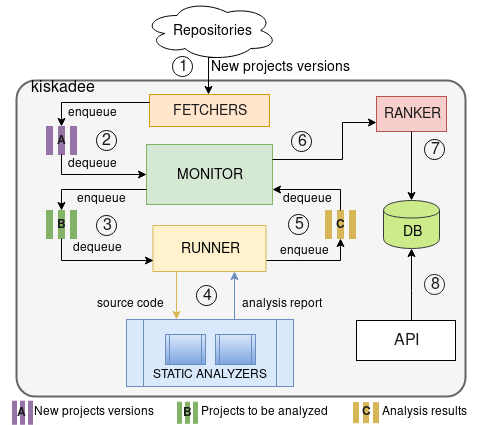
\includegraphics[width=.95\textwidth]{figures/kiskadee-overview} 
  \caption{kiskadee overview.}
  \label{fig:kiskadee_overview} 
\end{figure}

\section{kiskadee Design}
\label{sec:kiskadee}

\textit{kiskadee} downloads the source code of each version of a software it
monitors, runs a set of predefined static analyzers on it and stores the
outputs in a database using a common warnings report format. This common format
is needed because each static analyzer defines its own format to report
warnings after an analysis run is performed. The following sections establish
and justify our choices with respect to a common reporting language, multiple
static analyzers and software repositories.

\subsection{Common reporting language}

The problem of having a common reporting language for static analyzers was
discussed in a previous work. By applying the Ockham Sound Analysis
Criteria~\cite{black_sate_2016}, we designed a simplified common bug report
format to compare known bugs with bug reports from the tools evaluated with the
criteria. The criteria data and programs to reproduce results are available in
the SATE V Ockham Sound Analysis Criteria NIST Internal Report
\cite{black_sate_2016}, where the bug report formats specified can be retrieved
from and replicated. While the format was fit to perform the analysis, it was
designed on top of the criteria concepts and the tools used for the criteria,
which needed the following information:

\begin{itemize}
\item a specific location for the bug;
\item the type of the bug being reported (related to a CWE);
\item a code snippet with the buggy code;
\item information to identify false alarms on that code snippet.
\end{itemize}

To extract information from the used test suite (code snippets with known
flaws injected) to verify the soundness of the analyzed tools, an XML
format was defined. Listing~\ref{lst:ockham_xml} is an example of the format,
extracted from one of the files with Ockham results.  Although tools to extract
information from the format were developed and are available, no formal
definition of the format was described, since this format was used for this
specific version of the criteria.

\begin{lstlisting}[caption={Ockham Criteria XML bug report example},label={lst:ockham_xml}]
<?xml version='1.0' encoding='utf-8'?>
<sites>
  <file name="CWE369_Divide_by_Zero__int_fgets_divide_51b.c">
    <site type="div_by_zero" line="27" info="data" val="buggy">
      <code><![CDATA[printIntLine(100 / data);]]></code>
    </site>
    <site type="div_by_zero" line="38" info="data" val="good">
      <code><![CDATA[printIntLine(100 / data);]]></code>
    </site>
    <site type="div_by_zero" line="47" info="data" val="good">
      <code><![CDATA[printIntLine(100 / data);]]></code>
    </site>
  </file>
</sites>
\end{lstlisting}

To compare the findings of the evaluated tools with actual data from the test suite,
tool reports were parsed and converted to a very simple comma-separated values
(CSV) format containing \textit{file name}, \textit{line} and \textit{bug category
related to a CWE}. An example of this CSV format, extracted from the Ockham
Criteria results, is shown in Listing~\ref{lst:ockham_csv}.

\lstset{language=Python}
\begin{lstlisting}[caption={Ockham Criteria CSV bug report example},label={lst:ockham_csv}]
CWE121_Stack_Based_Buffer_Overflow__char_type_overrun_memcpy_01.c, 43, divByZero
CWE121_Stack_Based_Buffer_Overflow__char_type_overrun_memcpy_01.c, 62, divByZero
CWE121_Stack_Based_Buffer_Overflow__char_type_overrun_memcpy_02.c, 45, divByZero
CWE121_Stack_Based_Buffer_Overflow__char_type_overrun_memcpy_02.c, 73, divByZero
CWE121_Stack_Based_Buffer_Overflow__char_type_overrun_memcpy_02.c, 92, divByZero
CWE121_Stack_Based_Buffer_Overflow__char_type_overrun_memcpy_03.c, 45, divByZero
CWE121_Stack_Based_Buffer_Overflow__char_type_overrun_memcpy_03.c, 73, divByZero
CWE121_Stack_Based_Buffer_Overflow__char_type_overrun_memcpy_03.c, 92, divByZero
CWE121_Stack_Based_Buffer_Overflow__char_type_overrun_memcpy_04.c, 51, divByZero
CWE121_Stack_Based_Buffer_Overflow__char_type_overrun_memcpy_04.c, 79, divByZero
\end{lstlisting}

To rank warnings, we would like to have information on analyzed software
versions, which static analyzer performed the analysis, the version of the
analyzer, severity of the problem found, and the string message given by the
analyzer. All this information may be interesting for research or bug reporting
purposes. Thus, if we were to use the format we developed for the Ockham Criteria,
changes would be needed, both to the format and to the tools provided to work
with it.

Having a common report output was also discussed in Free Software development
communities. The Fedora Project\footnote{\url{fedoraproject.org}} Static
Analysis Special Interest
Group\footnote{\url{fedoraproject.org/wiki/StaticAnalysis}} designed a tool to
run static analyzers during the package build
process\footnote{\url{github.com/fedora-static-analysis/mock-with-analysis}}.
Although the tool itself is in its early development stages and is not ready
for usage in production, the developers
discussed\footnote{\url{lists.fedoraproject.org/archives/list/firehose-devel@lists.fedoraproject.org}}
a common report format for the static analyzers in their mailing lists. The
Debian project\footnote{\url{debian.org}} community also got involved in the
discussion and  after a few iterations of collaboration, \textit{firehose}, a
complete definition of a common warnings report format for static analyzers and
a set of tools to generate, parse, and verify the format, was created.
\textit{firehose} addresses the issues previously discussed, as analyzer name
and version, optional fields for severity, and complete warning messages.
Appendix \ref{ape:firehose} is a RELAX-NG schema describing the
\textit{firehose} format.

Since \textit{firehose} meets our needs, we decided to use it as our common
warning report format, eliminating the need
to design a new output format and develop the tools to
handle it, like parsers and generators. If we encounter the need to add new information to the
format, we assume that the flexibility of the XML language will allow us to
include our own modifications to firehose.

\subsection{Static analyzers}

The NIST Software Assurance Metrics and Tool Evaluation (SAMATE) project
provides a list of \textit{source code security
analyzers}\footnote{\url{samate.nist.gov/index.php/Source_Code_Security_Analyzers.html}},
which they define as static analyzers that \textit{examine source code to
detect and report weaknesses that can lead to security vulnerabilities}.

We want to run at least 3 different tools, to be able to rank warnings based on
their output. To choose which static analyzers to run for this study, we used
the following criteria:

\begin{enumerate}
  \item \textbf{The tools must be recommended by SAMATE as a static analyzer with focus on source code security.} The selected tools must be either in the list of tools recommended by SAMATE or in one of the lists of static analyzers SAMATE also recommends.
  \item \textbf{The tools must use different methods of analysis.} This way, source code will be analyzed from different perspectives, possibly reducing the number of false negatives.
  \item \textbf{The tools must be able to analyze C programming language code.} Different programming languages have different problems and we do not want to address this variable at the moment. Since software is often developed in the C programming language, we will use it for this research.
  \item \textbf{The tools must be licensed under a FLOSS license.} We do not want to study different proprietary software licenses nor contact developers to make sure we are allowed to perform this study. Also, by using FLOSS and releasing our source code with FLOSS licenses, we avoid legal issues and support Free Software.
\end{enumerate}

\textit{Frama-C} with its value analysis plug-in was the first choice, since it
was the tool used for the Ockham Criteria~\cite{black_sate_2016} and the
authors claim Frama-C is a sound tool, not producing false positives, which may
help on the ranking phase of this study. It uses abstract interpretation
techniques. Although Frama-C is not listed in the SAMATE recommended tools, it
is recommended by the Flawfinder
website\footnote{\url{dwheeler.com/flawfinder}}, one of the secondary tool
lists recommended by SAMATE. Next \textit{cppcheck} was chosen, which is a
static analyzer that works by matching on tokens, without deeper analysis
methods. This tool authors also claim to avoid generating false positives.
Finally, \textit{Clang Static Analyzer} works by performing inter-procedural
analysis on the source code and, differently from the other two selected tools,
the authors do not claim that this tool does not generate false positives.
Table \ref{tab:tool_selection} shows how each of the selected tools complies
with the selection criteria.

\begin{table}
  \centering
  \begin{tabular}{|c|c|c|c|c|}
    \hline
    \textbf{Tool} & \textbf{Recommended by} & \textbf{analysis method} & \textbf{C?} & \textbf{License}\\
    Frama-C & Flawfinder & abstract interpretation & yes & LGPLv2\\
cppcheck & SAMATE & token matching & yes & GPLv3\\
Clang Static Analyzer & SAMATE & inter-procedural & yes & NCSA and MIT\\
    \hline
\end{tabular}
  \caption{Selected static analyzers}
  \label{tab:tool_selection}
\end{table}

\subsection{Software repositories}

As previously mentioned, we want to work with GNU/Linux distributions. The
Debian Project has been developing a tool to run multiple static analyzers in
Debian repositories and return the reports in the \textit{firehose}
format\footnote{\url{debile.debian.net}}.  The tool is still in early development
(not in production), but we intend to use part of it with \textit{kiskadee} to
avoid replicating their work. Some development on it to provide options to
point to different repositories or remove non-Debian related code may be
necessary, which may result in contributions to the tool.

There may be advantages in pointing \textit{kiskadee} to the Fedora Project
repositories as well, since it updates packages in a faster pace than Debian,
and we want to analyze different versions of the same software. Since I am
closer to this project, hosting the tools in its infrastructure is also a
possibility.

\subsection{Architecture}

The system is composed of 4 modules, which are described in the sections
below. Figure \ref{fig:kiskadee_architecture} describes \textit{kiskadee}'s architecture.

%\begin{figure}[!h]
  %\centering
  %\includegraphics[width=.80\textwidth]{kiskadee_architecture} 
  %\caption{kiskadee architecture.}
  %\label{fig:kiskadee_architecture} 
%\end{figure}

\subsubsection{Monitor}

The Monitor module loads information of target packages from monitored
repositories and the latest previous version analyzed by kiskadee for each of these
packages. Then, it compares the versions of the packages available in the
repositories with the ones in the \textbf{kiskadee} database: if the version of
a package in the repositories is greater than the last analyzed version, it
writes a message in a queue informing there is a new version for that package.

\subsubsection{Runner}

The Runner module queries the shared queue for new messages. Whenever a message
is found, it uses the message information to download the new package version
and run the static analyzers on the downloaded package. Then it removes the
entry from the queue and sends the analyses reports to the Converter module.

\subsubsection{Converter}

This module receives the static analyses reports from the Runner module and
checks if they are valid firehose reports. If they are not, it converts them to
the firehose format. Finally, it saves the reports in the \textit{kiskadee}
database.

\subsubsection{Plugins}

kiskadee needs plugins to operate. Each plugin must implement
functions that define:

\begin{enumerate}
  \item which repository to monitor;
  \item how to monitor the repository;
  \item the message format in the queue that triggers the runner;
  \item which static analyzers to run and how to run them;
  \item how to convert an analyzer output to the firehose format.
\end{enumerate}

With this level of modularization, we can extend \textit{kiskadee} to perform
analysis with different static analyzers in different types of software
repositories.

\section{Ranking warnings}
\label{sec:ranking_warnings}

We will approach the problem of ranking multiple static analyzers warnings as a
\textit{learning to rank} problem~\cite{liu2009learning}. Learning to rank is
commonly applied in document retrieval problems, such as search engines.
Although some algorithms are designed for specific tasks, like ranking web
pages, there are learning to rank algorithms that can be applied in different
contexts. To select a proper learning to rank algorithm, literature on learning
to rank will be reviewed along with the papers selected in the structured
review described in Chapter \ref{cap:structured_review}.

To be able to rank the warnings taking into consideration some knowledge about
the performance of the tools, we may evaluate each of the tools used by
analyzing some set of known security flaws. Then, it is possible to match the
tool findings with the actual flaws, assessing the tools using metrics based on
false positive rate, true positive rate, and false negative rate. A set of
known security flaws may consist of real world software or artificial test
cases. In both cases, the set of known security flaws should either be provided
with a list of all the flaws it contains and their location, or have all its
flaws annotated. SAMATE provides the \textit{Software Assurance Reference
Dataset}\footnote{\url{samate.nist.gov/SARD}} (SARD), which is composed of a
few sets with thousands of known security flaws, published for research and
tool development purposes. Among these sets provided by SAMATE, there is one
test suite we can use to assess the static analyzers and train our model.
Juliet is an artificial C/C++ test suite with 61,387 test cases covering 118
different CWEs. Each test case contains a code snippet with an instance of a
specific CWE and another code snippet with a fix for that flaw.
% incluir snippet do juliet aqui?

With the analysis reports obtained by running the static analyzers on the set
of known security flaws, we can empirically select the features that we will
use for our model and train the model. Possible features are the tool that
triggered a warning, the rank of the warning in the tool that triggered it, the
criticality of the warning according to the tool, and the false negative rates
of the tools (we believe that, if a tool produces less false positives, it is
more conservative on its heuristics, thus, generates more false negatives as
well: that is why we want to verify if the false negative rate is a good
feature to rank the warnings). Although warning messages are different in each
static analyzer since there are no standards for warning messages and not all
of these tools adopt CWE terminology, it is possible to associate warnings
triggered by the same software flaw, even if it is by using simple heuristics,
like the location of each tool finding, which could also be used as a feature.

To validate our model, we will compare its accuracy against random ranking
algorithms, as seen in related works~\cite{kremenek2003z}.  Finally, we will apply
the model on the kiskadee database to rank each report on it. Afterwards, the model
can also be validated by manually gathering information from specific project
bug trackers or by manually analyzing each warning and verifying if the
warnings in the top of the reports are real flaws or false positives.

% Talvez não para agora, mas vc pode usar isso como parte do treinamento também.
We could also use the decay time of the warnings across versions to help
identifying false positives~\cite{kim_which_2007, penta_evolution_2008}, but
since we also propose a filter to display warnings introduced in specific
software versions, this would have no value whenever the filter is used.
Also, Tracking those warnings across versions would also increase the
complexity of our analysis.

To generate the reports to evaluate the static analyzers and train our machine
learning model, we will extend kiskadee to run static analyzers on Juliet as
well. This way, the data used for this research will also be available in the
kiskadee database.

\section{Visualization}
\label{sec:visualization}

Related works propose methods to identify bugs included or fixed in specific
software versions, as mentioned in Section \ref{history_review}.
Also, there are existing tools like
csdiff\footnote{\url{https://github.com/kdudka/csdiff}} that provide some
logic to parse static analyzer reports from different software versions and
list new and removed warnings. csdiff provides parsers for both cppcheck and
the Clang Static Analyzer; a parser for Frama-C would have to be written.

These tools and techniques could be used to filter warnings by version, so the
ranked warning list displayed to the user will be a subset of the whole
analysis report, containing only the warnings introduced in a specific version
of the analyzed software. This could also aid in identifying false positives,
as proposed by Kim et al.~\cite{kim_which_2007}, since the false positives are
not fixed between versions.

For our visualization tool, we will assess the effort needed to patch csdiff
to suit our needs and the effort to reproduce related works. Then we will
apply the technique that requires less effort to identify the warnings introduced
in a specific version of a package.

\section{Expected Results}

In Section \ref{sec:contributions} we proposed four major contributions.
Contributions \textbf{C1} and \textbf{C2}, referring to the continuous static
analysis tool and the static analysis warnings database, will be achieved with
kiskadee, our continuous static analysis system, as described in Section
\ref{sec:kiskadee}. Contribution \textbf{C3} will be achieved empirically, by
studying the data collected by the kiskadee database and finding relevant
factors to rank the warnings, as described in Section
\ref{sec:ranking_warnings}. By successfully ranking the warnings, which will be
verified by comparing the ranking algorithm with other ranking methods, we will
answer our research question and confirm hypotheses \textbf{H1} and
\textbf{H2}. Finally, Contribution \textbf{C4} will be achieved by using
existing methods to identify warnings introduced in specific versions of the
analyzed software packages. Achieving all the contributions here described, the
main objective of this masters thesis will be met, providing means to reduce
efforts to include static analysis in software development cycle.

%%%%%%%%%%%%%%%%%
%%%%%%%%%%%%%%%%%
%%%%%%%%%%%%%%%%%
%%%%%%%%%%%%%%%%%
%%%%%%%%%%%%%%%%%
%%%%%%%%%%%%%%%%%
%%%%%%%%%%%%%%%%%

\section{Continuous Static Analysis with kiskadee}
\label{sec:continuous_static_analysis}

In Free/Libre and Open Source Software (FLOSS) projects, a common source of bug reports are the GNU/Linux
distributions. These distributions ship thousands of software projects, which
they call packages. Distribution developers refer to the projects that maintain
the software they ship in the distribution as \textit{upstream}.  It is not
unusual for distribution developers to report bugs in upstream projects or to
send patches to fix bugs found by their distribution users or during the
packaging process.

By continuously running multiple static analyzers in several of these packages,
i.e., once for each version of the package, we can create a database of static
analysis reports on software projects of different sizes and application
domains. Developers can then use the information in this database to find and
act on software flaws.

\begin{figure}[hbt]
\centering
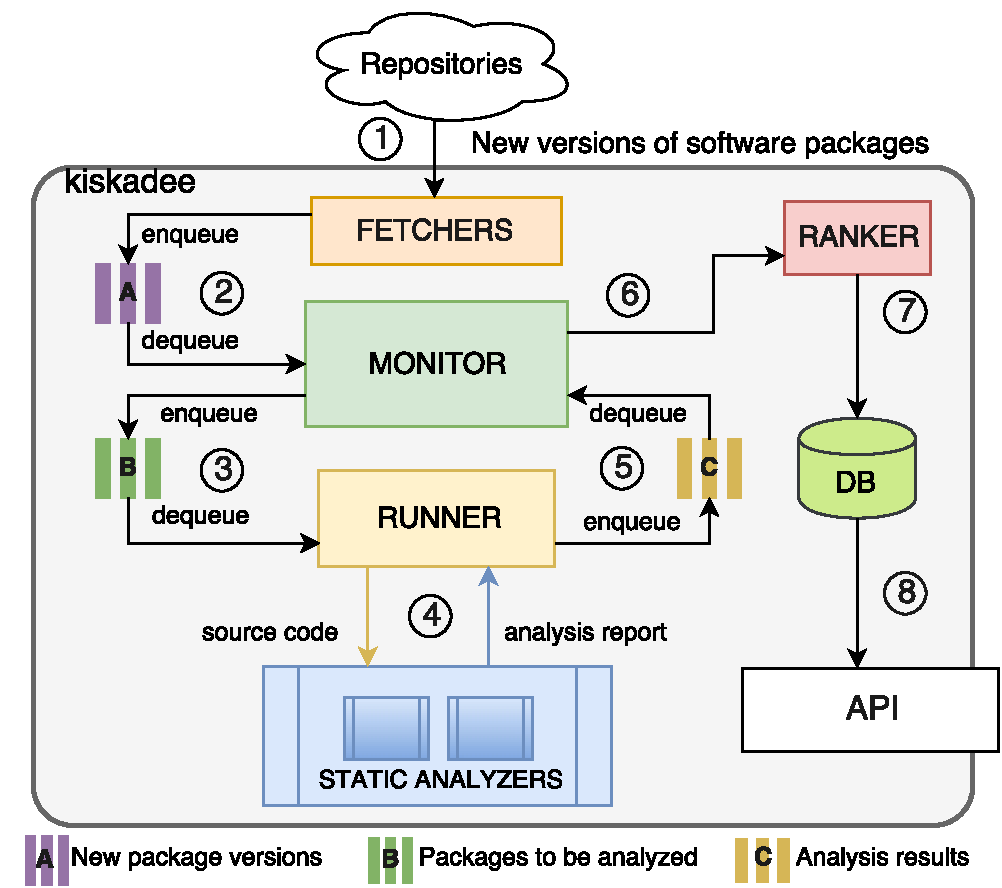
\includegraphics[width=.7\textwidth]{figures/kiskadee-overview.pdf}
  \caption{kiskadee design overview.}\label{fig:kiskadee:overview}
\end{figure}

We chose to use GNU/Linux distributions due to the high amount of software
packages available and the well-defined and documented interfaces they provide
to download the latest versions of these packages. It is also an advantage that
the cultural norm for GNU/Linux distribution developers is to report (and often
propose fixes for) bugs. Therefore, using their repositories for this work may
provide a broader user base for the tools and techniques developed in this
research.

To continuously run static analysis on software packages and handle the false
alarms generated by these analyses, we developed \textit{kiskadee}.
Figure~\ref{fig:kiskadee:overview} represents kiskadee's architecture overview,
where the numbers denote its execution flow. In steps (1) and (2), kiskadee
monitors software repositories for new releases. In step (3), kiskadee
downloads the source code of each new software version in a repository it
monitors and runs a set of predefined static analyzers on it in step (4). In step (5),
kiskadee translates each static analyzer report to a common warnings report format.
This common format is needed because each static analyzer defines
its unique format to report warnings. In step (6), kiskadee ranks the warnings
based on their probability of being real bugs, where warnings on the top have a
higher probability of being real bugs and warnings on the bottom are more
likely to be false positives. This ranking step is performed with a
classification model, described in Section~\ref{sec:ranking}. The ranked
warnings are then saved in a database in step (7), using kiskadee's common
warning report format.  Finally, in step (8), kiskadee provides an API consumed
by a visualization tool to display the ranked warnings filtered by package
versions. The information provided can be used either by distribution developers to
evaluate and report possible bugs upstream or by upstream developers
themselves. Researchers can also use kiskadee's database in different contexts.

FLOSS development communities have been discussing a common static analysis
report output format. The Fedora Project Static Analysis Special Interest Group
\cite{fedora:static:sig} designed a tool to run static analyzers during the
package build process \cite{fedora:mockwithanalysis}.  Although the tool itself
is in its early development stages and not ready for usage in production, the
developers discussed \cite{fedora:mlist} a common report format for the static
analyzers in their mailing lists. After a few iterations, with Debian Project
developers collaboration, they created \textit{Firehose}, a complete definition
of a common warnings report format for static analyzers and a set of tools to
generate, parse, and verify this format.  We use \textit{Firehose} as kiskadee's
common warning report format, eliminating the need to design a new format and
to develop the tools to handle it, like parsers and generators.

\textit{kiskadee} was run with three static analysis tools to generate the
warnings data set for our experiments. The Criteria to select the tools were:
\begin{enumerate}
  \item The tool must be able to examine C/C++ code for security flaws (e.g., buffer overflows, null pointer dereferences); and
  \item the tool source code must be released under an FLOSS license.
\end{enumerate}
Criterion~1 ensures the tool can analyze a subset of the test cases in our data
set, introduced in Section~\ref{sec:ranking}, whereas criterion 2 preserves us
from disputes by tool vendors regarding the analysis of the results (such as
allegations of sub-optimal tool calibration or detrimental calculation
methodology). FLOSS tools also simplify the process of retrieving string
constructs for static analyzer warning messages and categories when necessary,
since we can verify their source code. Following the criteria, the static
analyzers selected were \emph{Clang Static Analyzer} (version 3.9.1),
\emph{Cppcheck} (version 1.79), and \emph{Frama-C} (version 1.14 with the value
analysis plugin activated).

Fedora Project uses an external system to monitor the software projects they
distribute. Anitya \cite{anitya} maps upstream projects to distribution package
names. Whenever a new version of an upstream project is released, Anitya
publishes the new release in a Fedora infrastructure publish-subscribe system
where other systems in the distribution infrastructure can handle it.
New software versions are published by Anitya as soon as they are released
upstream. Analyzing these new software versions with kiskadee as early as they
are released allows the distribution developers to address potential bugs found
by kiskadee before the software is shipped to final users. Therefore, kiskadee
monitors packages by reading information published by Anitya in the Fedora
infrastructure publish-subscribe system.

kiskadee can point to other software repositories as well through its plugin
architecture (kiskadee's fetchers). Each fetcher must implement functions that
define which repository to monitor, how to monitor it, and which static
analyzers to run for that repository. Hence, we can extend \textit{kiskadee} to
run different static analyzers for different software repositories or GNU/Linux
distributions.
